
\begin{enumerate}
    \item The intersection of the lines is given by 
    
\begin{align}
    \myvec{3 & -4 \\ 3 & 9}\vec{x}=
\myvec{-6 \\ 9}
\end{align}
for which, the augmented matrix is
\begin{align}
    \myvec{3 & -4 & -6\\
           3 & 1 & 9}
\end{align}
which  can be reduced as 
 \begin{align}
     \myvec{3 & -4 & -6\\
           3 & 1 & 9}
    \xleftrightarrow[R_1 \leftarrow R_2]
    {R_2 \leftarrow R_1}
    \myvec{3 & 1 & 9\\
          3 & -4 & -6}\\
          \xleftrightarrow{R_1 \leftarrow \frac{R_1}{3}}
    \myvec{1 &\frac{1}{3}&3\\
        3&-4&-6}\\
        \xleftrightarrow{R_2\leftarrow R_2-3R_1}
    \myvec{1&\frac{1}{3}&3\\0&-5&-15}\\
    \xleftrightarrow{R_2\leftarrow \frac{1}{5}R_2}
    \myvec{1&\frac{1}{3}&3\\0&1&3}\\
    \xleftrightarrow{R_1\leftarrow R_1-\frac{1}{3}R_2}
    \myvec{1&0&2\\0&1&3}
 \end{align}
\begin{align}
\therefore \vec{P}=\myvec{2\\3}
\end{align}
is the point of intersection of the lines and the vertex of the triangle formed by the two lines with x-axis as base.
\item 
The     equation of the x axis is 
    \begin{align}
        \myvec{0&1}\vec{x}=0
    \end{align}
    Thus, the intersection of \eqref{linform/2006/2/11/eq:1} with the x axis is given by the set
     \begin{align}
        \myvec{3&-4}\vec{x}=-6\\
        \myvec{0&1}\vec{x}=0
    \end{align}
    The augmented matrix for above is
\begin{align}
    \myvec{3 & -4 & -6\\
           0 & 1 & 0}
\end{align}
which  can be reduced as 
\begin{align}
    \myvec{3 & -4 & -6\\
           0 & 1 & 0}
    \xleftrightarrow {R_1 \leftarrow \frac{1}{3}R_1}
    \myvec{1 & \frac{1}{3} & 3\\
          0 & 1 & 0}\\
          \xleftrightarrow{R_1 \leftarrow R_1 + \frac{4}{3}R_2}
    \myvec{1 &0&-2\\
        0&1&0}\\
\end{align}
\begin{align}
\therefore \vec{Q}=\myvec{-2\\0}
\end{align}
is the point of intersection of the line \eqref{linform/2006/2/11/eq:1} with the x axis.
\item Similarly, the intersection of \eqref{linform/2006/2/11/eq:2} with the x axis is given by the set

 \begin{align}
        \myvec{3&1}\vec{x}=9\\
        \myvec{0&1}\vec{x}=0
    \end{align}
 with    augmented matrix 
\begin{align}
    \myvec{3 & 1 & 9\\
           0 & 1 & 0}
\end{align}
Twhich  can be reduced as 
\begin{align}
    \myvec{3 & 1 & 9\\
           0 & 1 & 0}
    \xleftrightarrow {R_1 \leftarrow \frac{1}{3}R_1}
    \myvec{1 & \frac{1}{3} & 3\\
          0 & 1 & 0}\\
          \xleftrightarrow{R_1 \leftarrow R_1 - \frac{1}{3}R_2}
    \myvec{1 &0&3\\
        0&1&0}\\
\end{align}
resulting in 
\begin{align}
    \vec{R}=\myvec{3\\0}
\end{align}
as the point of intersection of the line \eqref{linform/2006/2/11/eq:2} with the x axis.

    % \begin{align}
    %     \vec{P}=\myvec{2\\3}\\ \vec{Q}=\myvec{-2\\0}\\ \vec{R}=\myvec{3\\0}\\
    % \end{align}
    % represent the vertices of the triangle formed by the lines \eqref{linform/2006/2/11/eq:1} \& \eqref{linform/2006/2/11/eq:2}
    % with the X-axis.\\\\
    %     P is the vertex of the triangle.
    %     Q is the point at which \(3x-4y+6=0\) meets the X-axis.\\
    %     R is the point at which \(3x+y-9=0\) meets the X-axis.\\
\end{enumerate}
These points are then plotted in Fig. \ref{linform/2006/2/11/Fig 1.1} for verification.
\begin{figure}[h]
\centering
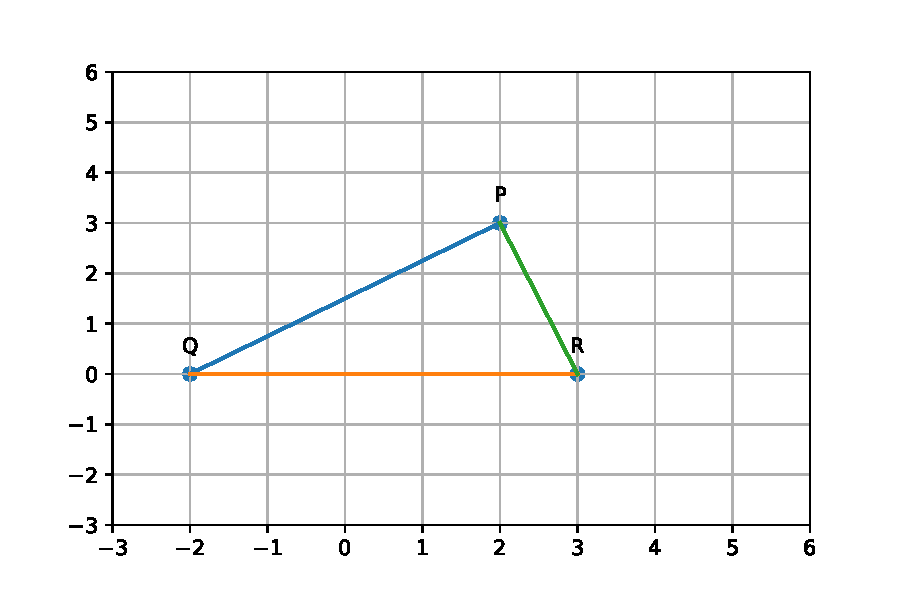
\includegraphics[width=\columnwidth]{linear_forms/solutions/2006/2/11/Figures/line.pdf}
\caption{Two lines representing given equations meet at point $\myvec{2 & 3}$ }.
\label{linform/2006/2/11/Fig 1.1}
\end{figure}
%\end{enumerate}